\documentclass[a4paper,12pt,leqno,titlepage]{article}
\usepackage{hyperref} %linkitys
\usepackage{graphicx}
\usepackage{listings}
\usepackage{moreverb}
\usepackage{amsmath}
\usepackage{amsthm}
\usepackage[english]{babel}
%\usepackage[finnish]{babel}
\usepackage{ucs}
\usepackage[utf8x]{inputenc}
\usepackage{amssymb}

\usepackage{algorithm2e}
\newcommand{\R}{\mathbb{R}} %lukujoukkosymbolit
\newcommand{\C}{\mathbb{C}}
\newcommand{\Q}{\mathbb{Q}}
\newcommand{\N}{\mathbb{N}}
\newcommand{\Z}{\mathbb{Z}}
\newcommand{\logM}{\mathcal{M}}
\newcommand{\bigO}{\mathcal{O}}
\setlength{\parindent}{0pt} %kappalejakoa
\setlength{\parskip}{2ex}
\newcommand{\compcent}[1]{\vcenter{\hbox{$#1\circ$}}}
\newcommand{\comp}{\mathbin{\mathchoice
{\compcent\scriptstyle}{\compcent\scriptstyle}
{\compcent\scriptscriptstyle}{\compcent\scriptscriptstyle}}}

%\hyphenpenalty=750
%\setlength{\emergencystretch}{1.5 em} % Tavutusasetukset suomen kielelle

\hypersetup{
pdfborder = {0 0 0 0}, %linkkien värejä etc kikkailua
colorlinks = true,
linkcolor = black,
urlcolor = blue,
citecolor = red,
}


\usepackage{lastpage} %sivumäärä alaviitteeseen
\usepackage{fancyhdr}

\pagestyle{fancy}
\cfoot{Page \thepage/\pageref{LastPage}} % \\ Opiskelijanumero 013126382}


\begin{document}
\begin{titlepage}
\title{Data structures project, \\
Implementation document}
\author{Heikki Haapala and Aleksi Markkanen\\
Student numbers 014090190 and 013126382\\
\pageref{LastPage} pages}
\date{\today}
\end{titlepage}
\maketitle
\pagebreak
\tableofcontents
\pagebreak



\begin{comment}
Toteutusdokumentti

Ohjelman yleisrakenne
Saavutetut aika- ja tilavaativuudet (m.m. O-analyysi pseudokoodista)
Suorituskyky- ja O-analyysivertailu (mikäli työ vertailupainotteinen)
Työn mahdolliset puutteet ja parannusehdotukset
Lähteet
\end{comment}

\section{Structure of the Program}
We divided the code into five different \emph{Java} source packages: algorithms, comparators, datastructures, graphics and main.

Package \emph{algorithms} contains an interface \texttt{Algorithm} which the algorithms will implement.
Only one method is specified, namely \texttt{useAlgorithm}.
All other methods are declared \texttt{private}.

\emph{Comparators} contains only one class, \texttt{AngleComparator}.
It implements a comparator for the \texttt{Point2D.Double} class, in which the points are sorted in ascending order by their polar angles.
This method of sorting is used by the \emph{Gift-wrapping algorithm}.

Package \emph{datastructures} contains our implementation of the linked list.
We implemented methods to add and remove points, to sort the list and to check wether a given object is in the list.
The list also knows its length.

The \emph{graphics} package contains code necessary to draw the results on the screen.
In the \emph{main} package we placed all other program logic, i.e. input parameters, reading and writing to and from files and so on.


\pagebreak
\section{Attained Computational Complexity}
In the definitions document, we aimed for the best possible time complexities for our algorithms of choice.
However, for simplicity, we decided to settle for $\bigO(n)$ space complexity.
This way, we could generate a new linked list for the points of the convex hull.
This also reduced the complexity of our algorithms, especially the Quickhull algorithm.


\subsection{$\bigO$-analysis of the pseudocode}
\subsubsection{QuickHull}
\begin{algorithm}[H]
 \SetAlgoLined
\SetKwFunction{QuickHull}{QuickHull}

\QuickHull{$S$}

\KwData{List $S$ of points on a plane}
 \KwResult{List $H$ of points that form the convex hull of $S$}
\BlankLine
Find the points $A$ and $B$ that have the minimum and maximum values for $x$-coordinates, respectively.
These points are bound to be a part of the convex hull.
 
Divide $S$ into $S_1$ and $S_2$ so that points in $S_1$ and $S_2$ lie on the opposite sides of the line $AB$.

$H \leftarrow \{\}$.

$H = \text{FindHull}(S_1,A,B) \cup \text{FindHull}(S_2,B,A)$ 
\BlankLine
 
\caption{Core method}
\end{algorithm}

\begin{algorithm}[H]
\SetAlgoLined
\SetKwFunction{FindHull}{FindHull}

\FindHull{$S,A,B$}

\KwData{List $S$ of points on a plane, Point $A$, Point $B$}
\KwResult{List $H$ of points that form the convex hull of $S$ and are on the right of the line $AB$}
\BlankLine
\If{$S$ is empty}{return $A,B$}
Find $C = \text{argmax dist}(AB,C)$

Divide $S$ into $S_1$ and $S_2$ so that points in $S_1$ lie on the right side of $AC$ and points in $S_2$ lie on the right side of $BC$.
The rest of the points can be discarded.

return FindHull$(S1,P,C) \cup$ FindHull$(S2,C,Q)$.
\BlankLine
\caption{FindHull method}
\end{algorithm}
At first, it would seem that the time complexity of the recursive method is of order $\bigO(n^2)$.
While this is true for some datasets, usually the recursive method discards many points with each iteration and
thus brings the \emph{average-case time complexity} down to $\bigO(n\log n)$.

\subsubsection{Gift-wrapping}
The following pseudocode specifies the Jarvis' march algorithm\cite{GW}.

\begin{verbatim}
jarvis(S)
pointOnHull = leftmost point in S
i = 0
repeat
 P[i] = pointOnHull
 endpoint = S[0]         // initial endpoint for a candidate edge on the hull
  for j from 1 to |S|-1
   if (endpoint == pointOnHull) or (S[j] is left of line from P[i] to endpoint)
     endpoint = S[j]   // found greater left turn, update endpoint
  endfor
  i = i+1
  pointOnHull = endpoint
until endpoint == P[0]      // wrapped around to first hull point
\end{verbatim}

The inner loop of the pseudocode is run for each input point.
Thus, its time complexity is of order $\bigO(n)$. 
However, the outer loop is iterated over the hull points.
If there are $h$ hull points, the total time complexity is $\bigO(nh)$.
This is a so-called \emph{output-sensitive} algorithm.


\subsubsection{Graham scan}
Graham scan is given by the following pseudocode\cite{GS}:

We begin by defining an auxilliary function. \begin{verbatim}
function ccw(p1, p2, p3):
    return (p2.x - p1.x)*(p3.y - p1.y) - (p2.y - p1.y)*(p3.x - p1.x)
\end{verbatim}

Now we can write the graham scan in a simpler form.

\begin{verbatim}
let N           = number of points
let points[N+1] = the array of points
swap points[1] with the point with the lowest y-coordinate
sort points by polar angle with points[1]

# We want points[0] to be a sentinel point that will stop the loop.
let points[0] = points[N]

# M will denote the number of points on the convex hull.
let M = 1
for i = 2 to N:
    # Find next valid point on convex hull.
    while ccw(points[M-1], points[M], points[i]) <= 0:
          if M > 1:
                  M -= 1
          # All points are collinear
          else if i == N:
                  break
          else
                  i += 1

    # Update M and swap points[i] to the correct place.
    M += 1
    swap points[M] with points[i]

\end{verbatim}

The actual algorithm has the time complexity $\bigO(n)$, but since it is necessary to sort the input first,
it is dominated by the time complexity $\bigO(n\log n)$ of our \emph{Mergesort} implementation. 

\pagebreak
\section{Comparing the Different Algorithms}

\pagebreak
%\section{Ohjelman toiminnan empiirisen testauksen tulosten esittäminen graafisessa muodossa}
\section{Graphical Presentation of the Results of the Empirical Testing of the Correctness of the Program}
\begin{figure}[h!]
\caption{A picture of a gull.} %convex hull}
\centering
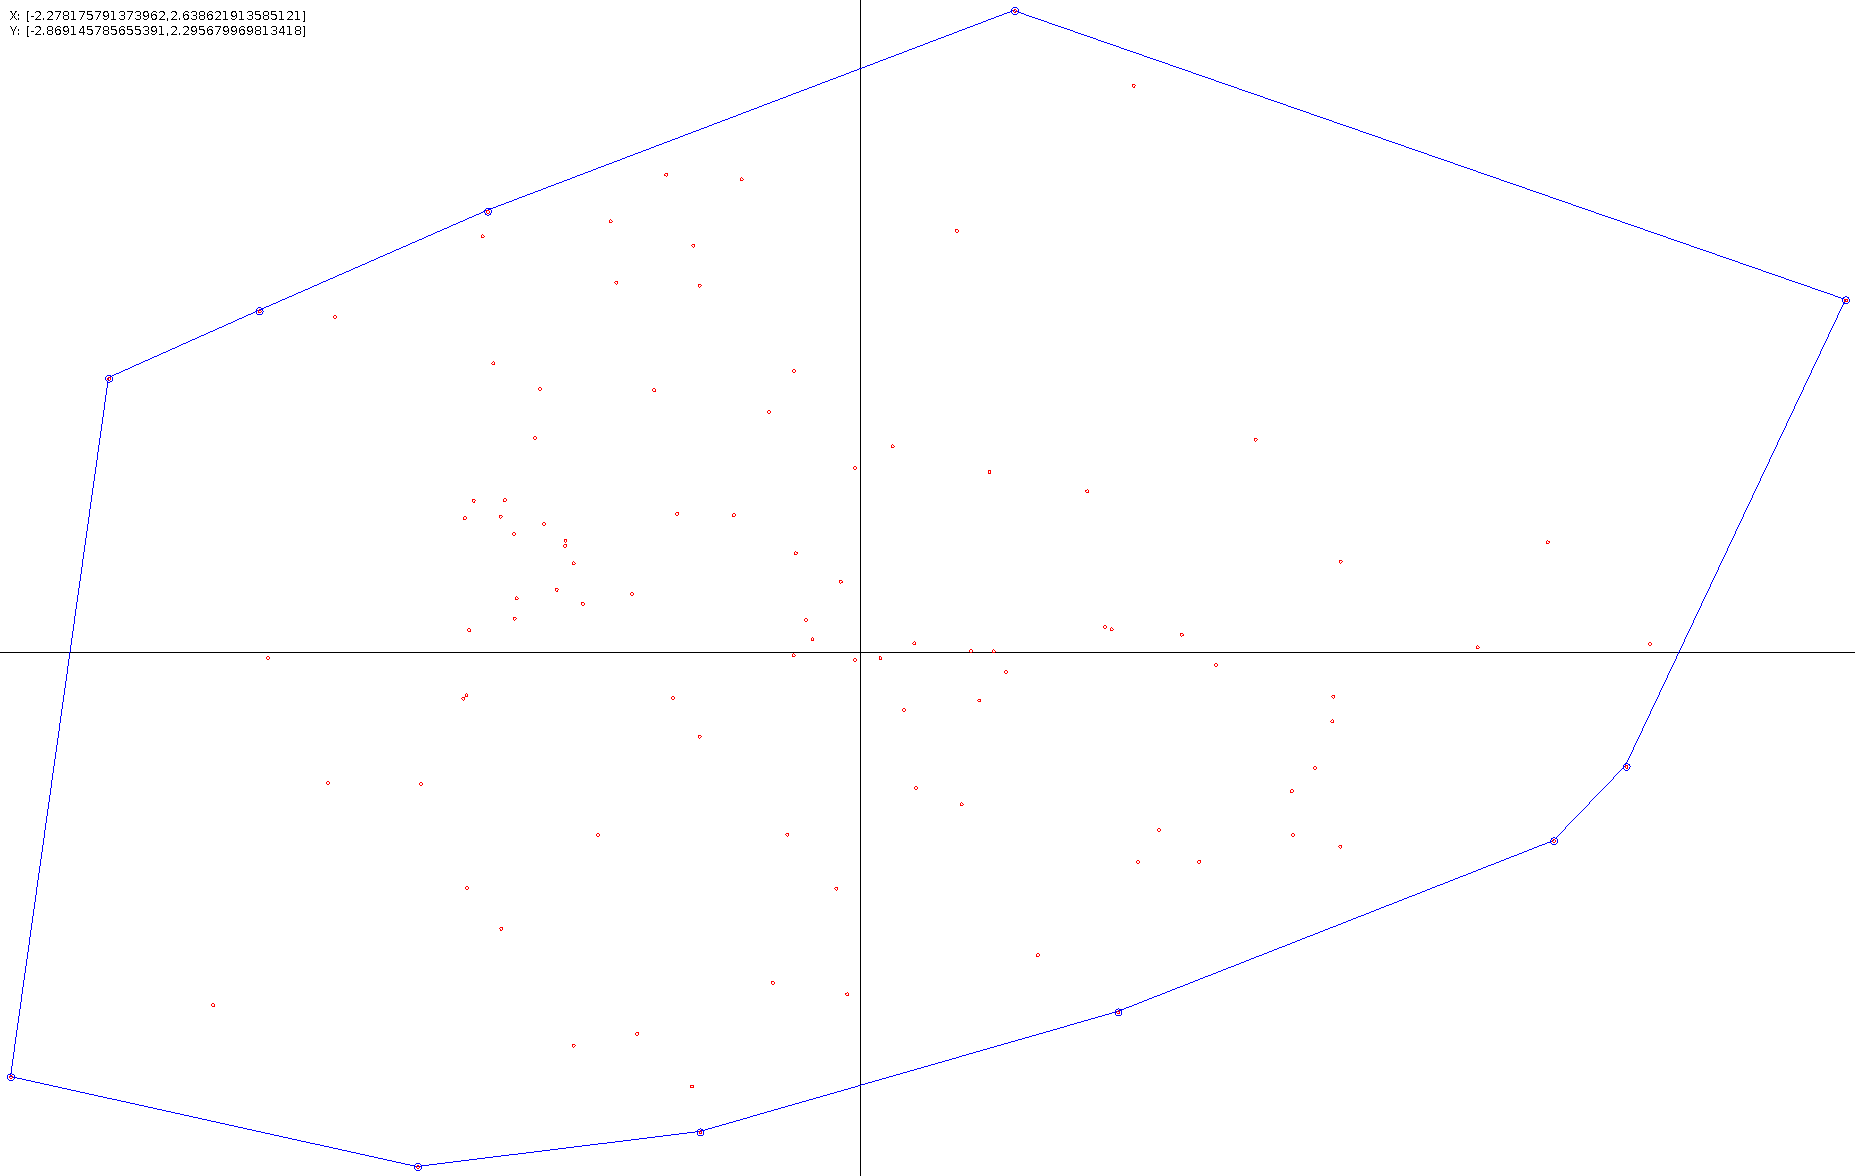
\includegraphics[width=\textwidth]{gull.png}
\end{figure}

\pagebreak


\begin{thebibliography}{9}
\bibitem{wiki}

Convex hull algorithms,

Wikipedia, the free encyclopedia

\url{http://en.wikipedia.org/wiki/Convex_hull_algorithms}

\bibitem{GW}
Gift Wrapping Algorithm,

Wikipedia, the free encyclopedia

\url{http://en.wikipedia.org/wiki/Gift_wrapping_algorithm}

\bibitem{GS}
Graham Scan,

Wikipedia, the free encyclopedia

\url{http://en.wikipedia.org/wiki/Graham_scan}

\end{thebibliography}

\end{document}
